\documentclass[letterpaper, 10 pt, conference]{ieeeconf}
%\documentclass[a4paper, 10pt, conference]{ieeeconf}

\IEEEoverridecommandlockouts
\overrideIEEEmargins

% The following packages can be found on http:\\www.ctan.org
\usepackage{graphicx} % for pdf, bitmapped graphics files
%\usepackage{epsfig} % for postscript graphics files
%\usepackage{mathptmx} % assumes new font selection scheme installed
%\usepackage{times} % assumes new font selection scheme installed
\usepackage{amsmath} % assumes amsmath package installed
\usepackage{amssymb}  % assumes amsmath package installed

\usepackage{url}
\usepackage{ae} % Nice Slovak symbols
\usepackage{listings,lstautogobble} % Nice MATLAB source code
\usepackage{matlab-prettifier}


\newcommand{\polydegree}{n}




\title{\LARGE \bf
A software package for MPC design and tuning: MPT+
}

\author{Juraj Holaza, Lenka Gal\v{c}\'{i}kov\'{a}, Juraj Oravec, Michal Kvasnica
	\thanks{Authors are with Faculty of Chemical and Food Technology,
		Slovak University of Technology in Bratislava, 812~37 Bratislava, Slovakia,
		\texttt{juraj.holaza@stuba.sk}}
}


\begin{document}



\maketitle
\thispagestyle{empty}
\pagestyle{empty}

\begin{abstract}

The industrial implementation of the model predictive control (MPC) is driven by the necessity to design, tune, and validate the constructed control policy. 
We present a novel software toolbox for advanced model predictive control (MPC) design extending the \texttt{Multi-Parametric toolbox} (\texttt{MPT}).  Particularly, \texttt{MPTplus} introduces several advanced MPC controller design methods, including memory-efficient explicit Tube MPC design, Tube MPC controller with the limited rate of control actions, and a polynomial approximation of the $1-$, $\infty-$norm-based explicit control law. The benefits of the proposed toolbox are demonstrated using the both, numerical simulations and the laboratory implementation on the device with a fast dynamics.  

\end{abstract}

\section{Introduction}
\label{sec:introduction}

% [ TOOD: Write an Introduction ]
% [ TOOD: Introduce MPC ]
Although the model predictive control (MPC)~\cite{M00, B17} provides an optimal control policy under various physical and performance constraints, its industrial implementation is still under its significant relevance~\cite{QB03}. 
Introducing multi-parametric programming into MPC design framework~\cite{BM02} gained its potential by reducing the runtimes and requirements on the advanced software, pushed the MPC implementation towards the industrial embedded hardware, see~\cite{PK21}. Moreover, the construction of the explicit solution map in the form of the piece-wise affine (PWA) function enables rigorous certification of the control law. 
%
Although the MPC has been intensively studied in past three decades, there are still challenges worth addressing to spread its industrial implementation. Such a development is highly dependent on the tailored validation tools. 
% MOVED
The MPC design problem is addressed in plenty of well-developed software tools. Most of the packages provide dedicated built-in solvers, and the other delegate the optimization problem to third-party solvers. 

Following is a brief review of the MPC design software limited just for the tools offering an interface for the \texttt{MATLAB}\footnote{\texttt{MATLAB}, MathWorks, Inc.: \texttt{\url{https://www.mathworks.com}}} programming environment. We refer the reader to~\cite{KF18,LT17,HS22}, 
% ~\cite{KF18,LT17, OSQP,QPALM,qpDUNES,Ferreau2014,HPIPM,CVXGEN,EJ21,HS22}, 
and the references therein, for the review on the tailored solvers and tools supporting MPC design and its evaluation using also other programming environments, e.g., \texttt{Python}\footnote{\texttt{Python}, Python Software Foundation: \texttt{\url{https://www.python.org}}}, \texttt{Julia} \footnote{\texttt{Julia}, JuliaLang.org: \texttt{\url{https://julialang.org}}}, etc. Such packages include QP-solvers \texttt{qpDUNES}~\cite{qpDUNES}, \texttt{QPALM}~\cite{QPALM}, \texttt{CVXGEN}~\cite{CVXGEN}, and tools that introduce distributed optimization \texttt{OSQP}~\cite{OSQP}, \texttt{ALADIN}-$\alpha$~\cite{EJ21}, to name a few. 
% \texttt{Python}~\cite{PYTHON}, \texttt{Julia}~\cite{JULIA}, etc.

Commercial \texttt{MPC Toolbox}~\cite{MPC_toolbox} for \texttt{MATLAB} addresses various classes of the MPC design problems, including the construction of the adaptive, explicit, gain-scheduled, and non-linear MPC controllers. This toolbox provides several built-in solvers and also a dedicated user interface \texttt{MPC Designer App} for the controller tuning. 
%
The non-linear MPC design problems are efficiently solved using the \texttt{ACADO Toolkit}~\cite{ACADO_Toolkit}. The non-convex optimization problem is solved by the sequential quadratic programming (SQP) approach.  \texttt{ACADO Toolkit} evaluates the library-dependent \texttt{C/C++} code and provides an interface for \texttt{MATLAB}. 
%
\texttt{CasADi}~\cite{CasADi} represents another toolbox suitable for the non-liner MPC design. This open-source package also provides interfaces for \texttt{MATLAB} and \texttt{Python}. 
%
The non-linear MPC can be designed also using the open-source toolbox \texttt{MATMPC}~\cite{MATMPC}. 
%
\texttt{YALMIP}~\cite{L04} toolbox is a widely-used modelling parser focused on the various classes of optimization problems, including non-convex optimization. \texttt{YALMIP} provides also support for the MPC design problems. 
%
Similar to \texttt{YALMIP} toolbox, the \texttt{CVX}~\cite{GB08} is focused on modelling of various classes of convex optimization problems suitable for MPC controller design. 

% [ TODO: Introduce MPT ]
The \texttt{Multi-Parametric Toolbox} (\texttt{MPT})~\cite{MPT3} for \texttt{MATLAB} represents a widely-used software package for the implicit (non-explicit) and explicit MPC design, multi-parametric optimization, and operations over the convex sets. \texttt{MPT} integrates many tools enabling efficient construction, tuning, and validation of the advanced MPC controllers. 

The industrial implementation of the MPC is limited by the runtime effort and advanced hardware/software requirements, especially in case of the implicit MPC, and memory consumption, limiting implementation of explicit MPC on the industrial embedded hardware. Therefore, the complexity reduction methods are of a high interest. 
% [ TODO: Introduce LowCom ]
\texttt{MPT} module \texttt{LowCom}~\cite{KH15} introduces the set of methods reducing the complexity of the explicit solution maps associated with the MPC controllers to minimize the runtimes and memory footprints. 
In this framework, the polynomial-based approximation of the explicit solution maps introduced in~\cite{KL11} represents a perspective technique to minimize the memory footprint, however, it is not widely-available in some user-friendly way, yet.

% [ TODO: Introduce Tube MPC ]
In both, implicit and explicit MPC design problems, the Tube MPC represents a natural step towards the stochastic and non-linear MPC design. Finally, due to the ability to handle the quantized control variables, Tube MPC is also a necessary tool in a highly relevant field of the encrypted MPC design using the cloud-computing services, e.g., see~\cite{DR18} and the related works.

% [ TODO: Main contributions]
This paper presents the \texttt{MATLAB} toolbox \texttt{MPTplus}~\cite{MPTplus} augmenting the features of the original \texttt{MPT} toolbox by the notable methods introducing: (i) the framework for the memory-efficient explicit Tube MPC design, (ii) limits on a rate of control actions for implicit/explicit Tube MPC design, and (iii) the polynomial approximation of any explicit MPC controller according to~\cite{KL11}. To demonstrate benefits of the proposed \texttt{MPTplus} for real-world applications, we analyze results of an extensive case study considering the implementation of designed MPC controllers on the laboratory device having a fast-dynamics called Flexy~\cite{CK19}. 

\section{Theoretical backgrounds}
\label{sec:tube_mpc_theory}

% [ TOOD: Write the theoretical backgrounds on Tube MPC, delta-U constraints, and polynomial approximation. ] 
This section briefly reviews the main theoretical backgrounds of the currently implemented methods: (i) original (rigid) Tube MPC design approach proposed in~\cite{MS05} and its formulation considering multi-parametric optimization, (ii) limited rates on the control actions, and (iii) polynomial approximation of explicit control law.

\subsection{Tube MPC design}
\label{sec:tube_mpc}

Given an uncertain linear time-invariant (LTI) system defined as follows:
\begin{eqnarray}
	\label{eq:ulti_system}
	x(t+T_{\mathrm{s}}) = A x(t) + B u(t) + E d(t), % \quad x(0) = x_{0},
\end{eqnarray}
where $t$ is the time sample of the discrete-time domain defined using a sampling time $T_{\mathrm{s}}$. $A \in \mathbb{R}^{n_{\mathrm{n}_{x}} \times n_{\mathrm{n}_{x}}}$ is system matrix, $B \in \mathbb{R}^{n_{\mathrm{n}_{x}} \times n_{\mathrm{n}_{u}}}$ is input matrix, such that the matrix pair $(A,B)$ is stabilizable. $E \in \mathbb{R}^{n_{\mathrm{n}_{x}} \times n_{\mathrm{n}_{w}}}$ is disturbance matrix, $x \in \mathbb{R}^{n_{\mathrm{x}}}$ is the vector of the system states, $u \in \mathbb{R}^{n_{\mathrm{u}}}$ is control action, $d \in \mathbb{D} \subset \mathbb{R}^{n_{\mathrm{x}}}$ is bounded additive disturbance such that $\mathbb{D}$ is compact set containing the origin. 
For the disturbance in~\eqref{eq:ulti_system} holds:
\begin{eqnarray}
	\label{eq:disturbance_set}
	w = E \, d, ~ w \in \mathbb{W}, ~ \mathbb{W} = \left\{ w \in \mathbb{R}^{n_{\mathrm{x}}} : \Vert w \Vert_{\infty} \leq w_{\max} \right\},
\end{eqnarray}
where $w_{\max} = \Vert E \, d \Vert_{\infty}$ is an upper bound for $\forall d \in \mathbb{D}$ satisfying $\mathbb{W} \supseteq E \, \mathbb{D}$ is the minimum volume hyper-box such that $\Vert w \Vert_{\infty} = w_{\max}$.

Consider, the uncertain LTI system in~\eqref{eq:ulti_system} is constrained by
\begin{eqnarray}
	\label{eq:constraints_x_u}
	x(t) \in \mathbb{X}, \quad u(t) \in \mathbb{U}, \quad \forall t \geq 0,
\end{eqnarray}
where $\mathbb{X} \in \mathbb{R}^{n_{\mathrm{x}}}$ and $\mathbb{U} \in \mathbb{R}^{n_{\mathrm{u}}}$ are polytopes containing origin in their strict interiors. 

The convex set denoted as a ``tube'' $\mathbb{T} \subset \mathbb{R}^{n_{\mathrm{x}}}$ is  constructed as an invariant approximations of the minimal robust positively invariant set using an algorithm described in~\cite{RK05}.

%By plugging the LQ-optimal controller into~\eqref{eq:ulti_system} and updating the additive disturbances per~\eqref{eq:disturbance_set}, we obtain an autonomous discrete-time uncertain system 
%\begin{equation}
%	\label{eq:autosys}
%	x(t+T_{\mathrm{s}}) = (A + BK)x(t) + w(t).
%\end{equation}
%Subsequently, if $\mathbb{T}$ is a robust positive invariant (RPI) set for~\eqref{eq:autosys}, then we have that following statement holds 
%\begin{eqnarray}
%	\label{eq:tube}
%	\left( A + B K \right) \mathbb{T} \oplus \mathbb{W} \subseteq \mathbb{T},
%\end{eqnarray}
%where $\oplus$ denotes the Minkowski sum.

%Obviously, $\mathbb{T}$ in \eqref{eq:tube} is constructed as the minimal RPI set to minimize the conservativeness of Tube MPC design.
%by:
%\begin{eqnarray}
%	\label{eq:tube_design}
%	\mathbb{T} = \sum_{i=0}^{\infty} \left( A + B K \right)^{i} \mathbb{W},
%\end{eqnarray}
%where $\Sigma$ represents a set addition. However, if the $K$ is not a dead-beat controller, then the minimal RPI set $\mathbb{T}$ does not necessarily lead to the polytope, see~\cite{MS05}. Therefore, $\mathbb{T}$ is designed as the outer approximation of the minimal RPI set.  


The conventional (rigid) Tube MPC design problem has the form~\cite{MS05}:
\begin{subequations}
	\label{eq:tmpc}
	\begin{eqnarray}
		\label{eq:tmpc_cost}
		\min_{\hat{u}_{0},\ldots,\hat{u}_{N-1}, \hat{x}_{0},\ldots,\hat{x}_{N} } \!\!\!\!\!\!\!\!\!\!\! &\,& \Vert \hat{x}_{N} \Vert_{P}^{2} + \sum_{k=0}^{N-1} \left( \Vert \hat{x}_{k} \Vert_{Q}^{2} + \Vert \hat{u}_{k} \Vert_{R}^{2} \right) \qquad \\
		\label{eq:tmpc_rpi}
		\mathrm{s.t.\!:} &\,& x(t) - \hat{x}_{0} \in \mathbb{T} , \\
		\label{eq:tmpc_model}
		&\,&  \hat{x}_{k+1} = A \hat{x}_{k} + B \hat{u}_{k} , \\
		\label{eq:tmpc_constraints_state}
		&\,& \hat{x}_{k} \in \mathbb{X} \ominus \mathbb{T} , \\
		\label{eq:tmpc_constraints_terminal}
		&\,& \hat{x}_{N} \in \mathbb{X}_{\mathrm{N}}, \\
		\label{eq:tmpc_constraints_input}
		&\,& \hat{u}_{k} \in \mathbb{U} \ominus K \, \mathbb{T} , 
%		\label{eq:tmpc_constraints_input_delta_k}
%		&\,& \Delta \hat{u}_{l} \in \mathbb{U}_{\Delta} \ominus K \, \mathbb{T} , \\
		%\label{eq:tmpc_constraints_input_delta_0}
%		&\,& \hat{u}_{k} + K ( x(t) - \hat{x}_{0} ) - u(t_{-}) \in \mathbb{U}_{\Delta} , \quad
	\end{eqnarray}
\end{subequations}
for $\forall k = 0, \dots, N-1$,  $\forall l = 1, \dots, N-1$, and for prediction horizon $N$. Vectors $\hat{u}_{k}$ and $\hat{x}_{k}$ are decision variables optimized w.r.t. the nominal LTI system in~\eqref{eq:tmpc_model}, without any perturbations of the disturbance $w$. 
The squared $2-$norm objective function in~\eqref{eq:tmpc_cost} is minimized for the symmetric positive definite penalty factors $Q \in \mathbb{R}^{n_{\mathrm{x}} \times n_{\mathrm{x}}}$, $R \in \mathbb{R}^{n_{\mathrm{u}} \times n_{\mathrm{u}}}$, $P \in \mathbb{R}^{n_{\mathrm{x}} \times n_{\mathrm{x}}}$. 
The stability and recursive feasibility of Tube MPC design problem in~\eqref{eq:tmpc} has been proved in~\cite{MS05}.

Finally, the control action $u(t)$ to be implemented into to the uncertain LTI system in~\eqref{eq:ulti_system} is given by the control law $\kappa : \mathbb{X}_{\mathrm{F}} \rightarrow \mathbb{U}$
\begin{eqnarray}
	\label{eq:tmpc_control_law}
	\kappa(x(t)) = \hat{u}_{0}^{\star} + K \left( x(t) - \hat{x}_{0}^{\star} \right),
\end{eqnarray}
where symbol $\star$ in the optimal solution of the MPC design problem in~\eqref{eq:tmpc} and the feasibility set $\mathbb{X}_{\mathrm{F}} \subseteq \mathbb{R}^{n_{\mathrm{x}}}$ of the optimized initial condition $\hat{x}_{0}$ of~\eqref{eq:tmpc} represents its domain. 

%Tube MPC is implemented in receding horizon fashion, i.e., just the first control action $u(t) = \kappa(x(t))$ is applied to the plant and the optimization problem in~\eqref{eq:tmpc} is re-computed in each control step. 

The actuators of the physical systems are often under limited rates on the control actions formulated by:
\begin{eqnarray}
	\label{eq:rate_constraints_x_u}
	\Delta u(t) = u(t) - u(t_{-}) \in \mathbb{U}_{\Delta} ,
\end{eqnarray}
where $\Delta u(t) = u(t) - u(t_{-})$ is the rate of control action and $\mathbb{U}_{\Delta} \in \mathbb{R}^{n_{\mathrm{u}}}$ is the corresponding convex set bounding the rates. Then, the Tube MPC design problem in~\eqref{eq:tmpc} is extended by the linear constraint having the form: 
\begin{eqnarray}
	\label{eq:tmpc_constraints_input_delta_0}
	\hat{u}_{k} + K ( x(t) - \hat{x}_{0} ) - u(t_{-}) \in \mathbb{U}_{\Delta} , 
\end{eqnarray}
leading to the augmented vector of parameters $[x(t)^{\top}, u(t_{-})^{\top}]^{\top} \in \mathbb{R}^{n_{\mathrm{x}} + n_{\mathrm{u}}}$, in case of the multi-parametric solution of~\eqref{eq:tmpc}.

%% OUTPUT TUBE MPC
%
%The output feedback Tube MPC design problem has the form:
%\begin{subequations}
%	\label{eq:tmpc_output}
%	\begin{eqnarray}
%		\label{eq:tmpc_output_cost}
%		\min_{\hat{u}_{0},\ldots,\hat{u}_{N-1}, \hat{x}_{0},\ldots,\hat{x}_{N} } \!\!\!\!\!\!\!\!\!\!\! &\,& \Vert \hat{x}_{N} \Vert_{P}^{2} + \sum_{k=0}^{N-1} \left( \Vert \hat{x}_{k} \Vert_{Q}^{2} + \Vert \hat{u}_{k} \Vert_{R}^{2} \right) \qquad \\
%		\label{eq:tmpc_output_rpi}
%		\mathrm{s.t.\!:} &\,& x(t) - \hat{x}_{0} \in \mathbb{T}_{\mathrm{x}} , \\
%		\label{eq:tmpc_output_model}
%		&\,&  \hat{x}_{k+1} = A \hat{x}_{k} + B \hat{u}_{k} , \\
%		\label{eq:tmpc_output_constraints_state}
%		&\,& \hat{x}_{k} \in \mathbb{X} \ominus \mathbb{T} , \\
%		\label{eq:tmpc_output_constraints_terminal}
%		&\,& \hat{x}_{N} \in \mathbb{X}_{\mathrm{N}}, \\
%		\label{eq:tmpc_output_constraints_input}
%		&\,& \hat{u}_{k} \in \mathbb{U} \ominus K \, \mathbb{T}_{\mathrm{x}} , \\
%		% \label{eq:tmpc_output_constraints_input_delta_k}
%		% &\,& \Delta \hat{u}_{l} \in \mathbb{U}_{\Delta} \ominus K \, \mathbb{T} , \\
%		\label{eq:tmpc_output_constraints_input_delta_0}
%		&\,& \hat{u}_{k} + K ( x(t) - \hat{x}_{0} ) - u(t_{-}) \in \mathbb{U}_{\Delta} , \quad
%	\end{eqnarray}
%\end{subequations}
%where $\forall k = 0, \dots, N-1$,  $\forall l = 1, \dots, N-1$, $N$ is prediction horizon.
%
%$\mathbb{T} = \mathbb{T}_{\mathrm{y}} \oplus \mathbb{T}_{\mathrm{x}}$

\subsection{Explicit Tube MPC}
\label{sec:explicit_mpc}

% [ TODO: Write about explicit Tube MPC. ]
The main benefit of explicit MPC is its ability to significantly speed up the real-time evaluation of the optimal control action by pre-computing the optimization problem in advance, see~\cite{BM02}. Simultaneously, the explicit solution provides the possibility for rigorous analysis, verification, and certification of the designed control law. 

The QP in~\eqref{eq:tmpc} can be reformulated into the explicit MPC design framework by evaluating the initial condition in~\eqref{eq:tmpc_rpi} exploring the set of admissible initial conditions: $\Theta = \mathbb{X} \ominus \mathbb{T}$. Then, the solution of corresponding multi-parametric QP (mpQP) returns also the convex set of feasible system states $\mathbb{X}_{\mathrm{F}} \subseteq \Theta$ defined as the explicit solution map:
\begin{eqnarray}
	\label{eq:tmpc_partition}
	\mathbb{X}_{\mathrm{F}} = \bigcup_{i}^{n_{\mathrm{r}}} \mathcal{P}_{i} ,
\end{eqnarray}
where $\mathcal{P}_{i}$ are polytopes, i.e., critical regions, and $n_{\mathrm{r}}$ is the total number of critical regions.

As the consequence, for $x(t) \in \mathcal{P}_{i}$ denoting $i$th critical region, holds control law in~\eqref{eq:tmpc_control_law} given in a form of
piece-wise affine (PWA) functions corresponding to the particular decision variables:
\begin{subequations}
	\label{eq:tmpc_control_law_pwa_particular}
	\begin{eqnarray}
		\label{eq:tmpc_control_law_pwa_particular_x}
		\hat{x}^{\star}(x(t)) \!\!\!\!&=&\!\!\!\! F_{\mathrm{x},i} \, x(t) + g_{\mathrm{x},i} \quad \text{if} \quad x(t) \in \mathcal{P}_{i}, \\
		\label{eq:tmpc_control_law_pwa_particular_u}
		\hat{u}^{\star}(x(t)) \!\!\!\!&=&\!\!\!\! F_{\mathrm{u},i} \, x(t) + g_{\mathrm{u},i} \quad \text{if} \quad x(t) \in \mathcal{P}_{i},
	\end{eqnarray}
\end{subequations}
where $F_{\mathrm{x},i}$, $F_{\mathrm{u},i}$, $g_{\mathrm{x},i}$, $g_{\mathrm{u},i}$ have appropriate dimensions. For further technical details see~\cite{BM02}. 
Analogous to~\cite{ZT14}, we re-formulate the control law of the explicit Tube MPC in~\eqref{eq:tmpc_control_law_pwa_particular} into the compact form:
\begin{eqnarray}
	\label{eq:tmpc_control_law_pwa}
	\kappa(x(k)) = \underbrace{ \left( K + F_{\mathrm{x},i} + F_{\mathrm{u},i} \right) }_{ F_{i} } x(k) + \underbrace{ \left( g_{\mathrm{u},i} - K g_{\mathrm{x},i} \right) }_{ g_{i} }.
\end{eqnarray}
We point out, that such a compact formulation significantly reduces the associated memory footprint necessary to store the PWAs compared to the conventional explicit formulation in~\eqref{eq:tmpc_control_law_pwa_particular}.  
%
To be specific, the feedback law in~\eqref{eq:tmpc_control_law_pwa} saves $3\,n_\text{x}$ double precision numbers per each critical region compared to the original form~\eqref{eq:tmpc_control_law_pwa_particular_x}.
%
%	The memory savings related to storage of the set of $n_{\mathrm{r}}$ matrix pairs $(F_{\mathrm{x},i}, F_{\mathrm{u},i})$ compared to $F_{i}$ is, roughly, decreased by factor 2, and further savings related to pairs of vectors $(g_{\mathrm{x},i}, g_{\mathrm{u},i})$ compared to $g_{i}$ corresponds to $( n_{\mathrm{r}} \times n_{\mathrm{x}} )$ double-precision numbers.

\subsection{Polynomial approximation of explict MPC}
\label{sec:polynomial}
This section briefly recalls the theoretical backgrounds of the polynomial approximation of explicit MPC~\cite{kvasnica_polynomial}. This approach provides a technique suitable for control applications where low computational effort is necessary, while stabilizing the system and satisfying the constraints. On the other hand, the polynomial approximation of control law is suboptimal. 

Let us consider the MPC optimization problem in the following form:
\begin{subequations}
	\label{eq:empc}
	\begin{eqnarray}
		\label{eq:empc_cost}
		\min_{u_{0},\ldots,u_{N-1}} \!\!\!\!\!\!\!\!\!\!\! &\,& \sum_{k=0}^{N-1} \left( \Vert x_{k} \Vert_{Q}^{p} + \Vert u_{k} \Vert_{R}^{p} \right) \qquad \\
		\label{eq:empc_rpi}
		\mathrm{s.t.\!:} &\,& x_0 = x(t), \\
		\label{eq:empc_model}
		&\,&  x_{k+1} = A x_{k} + B u_{k} , \\
		\label{eq:empc_constraints_state}
		&\,& x_{k} \in \mathbb{X} , \\
		\label{eq:empc_constraints_input}
		&\,& u_{k} \in \mathbb{U},
	\end{eqnarray}
\end{subequations}
where the properties of the parameters are adopted from optimization problem in~\eqref{eq:tmpc}. The norm is considered as $p \in \{1,\infty \}$, i.e., the cost function in~\eqref{eq:empc_cost} is linear. Then, by multi-parametric solving for all feasible $x_0 \in \mathbb{X}_{\mathrm{F}}$, the PWA explicit feedback control law is obtained in the form:
\begin{eqnarray}
	\label{eq:empc_control_law}
	u^{\star}(x(t)) \!\!\!\!&=&\!\!\!\! F_{i} \, x(t) + g_{i} \quad \text{if} \quad x(t) \in \mathcal{P}_{i}.
\end{eqnarray}
The aim of this complexity reduction approach is to approximate the PWA control law in~\eqref{eq:empc_control_law} with a polynomial:
\begin{eqnarray}
	\label{eq:poly_control_law}
	\widetilde{u}^{\star}(x(t)) \!\!\!\!&=&\!\!\!\! a_{1} \, x(t) + a_{2} x(t)^2 + \dots + a_{d} x(t)^\polydegree,
\end{eqnarray}
where $a =\{a_{1}, \dots, a_{d}\}$ are the coefficients of the polynomial and $\polydegree$ is the polynomial degree which is fixed and given in advance by the control engineer. Note, the polynomial degree $\polydegree$ directly dictates the memory footprint of the approximated control law in~\eqref{eq:poly_control_law} and at the same time affects the performance loss. Therefore, $\polydegree$ is the main tuning parameter of the method that trades-off the performance and the complexity reduction of~\eqref{eq:poly_control_law}.

Let us presume that there exists a PWA Lyapunov function $L$ for the considered closed-loop system $f_{\mathrm{CL}}$, i.e. controlled system~\eqref{eq:ulti_system} subject to the control law in~\eqref{eq:empc_control_law}, such that $L(f_{\mathrm{CL}}) \le \gamma L(x)$, $L(0) = 0$ for $\gamma \in [0,1)$ and $x$ is within the feasible set $\mathbb{X}_{\mathrm{F}}$, i.e., $x \in \mathbb{X}_{\mathrm{F}}$. Considering the controlled LTI system, Lyapunov function $L$ and fixed $\gamma$, the stabilizing ``tube'' can be constructed according to~\cite{tube_FCh}:
\begin{eqnarray}
	\label{eq:stab_tube}
	\mathcal{T}(L, \gamma) := \begin{Bmatrix}
		[x^\top, u^\top]^\top \, : \, u \in \mathbb{U}, x \in \mathbb{X}_{\mathrm{F}} , A x + B u \in \mathbb{X}_{\mathrm{F}} \\
		L(f_{\mathrm{CL}}) \le \gamma L(x)
	\end{Bmatrix} \! , \nonumber 
\end{eqnarray}
consisting of $i = 1, \dots, n_\mathrm{r}$ polytopes:
\begin{eqnarray}
	\label{eq:stab_tube_polytope}
	\mathcal{T}_i := \begin{Bmatrix}
		[x^\top, u^\top]^\top \, : \, [T_i^{\mathrm{x}}, T_i^{\mathrm{u}}] [x^\top, u^\top]^\top \le T_i^0		
	\end{Bmatrix}. 
\end{eqnarray}
If such a stabilizing Lyapunov function exists and a stability ``tube'' is constructed, then the polynomial coefficients $a$ are obtained by solving a Polya-filter-based linear program minimizing the suboptimality level of~\eqref{eq:poly_control_law} from its optimal counterpart~\eqref{eq:empc_control_law}, i.e., $\min(\Vert\widetilde{u}^{\star}(x(t))-	u^{\star}(x(t))\Vert^{p})$. For more detailed overview of the approximation procedure see~\cite{kvasnica_polynomial}.

%If a stabilizing Lyapunov function can be found and a stability tube can be constructed, then the following linear programming problem can be solved
%\begin{subequations}
%	\label{eq:LP_a}
%	\begin{eqnarray}
%		\label{eq:LP_a_cost}
%		&\,& \min_{a}  z(\cdot) \\
%		\label{eq:LP_a_const}
%		&\,& \mathrm{s.t.\!:\,\,} \rho^{\phi}(a,\lambda) \geq 0, i = 1, \dots n_{\mathrm{r}}, 
%	\end{eqnarray}
%\end{subequations}
%
%to find the polynomial coefficients $a$. Several formulations of the objective function \eqref{eq:LP_a_const} are possible. The most common alternative is to define $z(\cdot) = 0$ to solve a pure feasibility problem.


\section{The software package MPT+}
\label{sec:code}

% [ TOOD: Describe a software package. ]

%\subsection{MPT+}
%\label{sec:code_mptplus}

% [ TOOD: Describe an MPT+ package. ]
The \texttt{MPTplus} toolbox extends the functionality of the \texttt{MPT} toolbox~\cite{MPT3}. In this section, we introduce the novel features, including (i) efficient explicit Tube MPC controller construction, (ii) introducing incremental constraints into the Tube MPC design, and (iii) the general polynomial approximation of the PWA control law. 

\subsection{Installation}
\label{sec:installation}

The \texttt{MPTplus} toolbox is freely available at \texttt{GitHub}\footnote{\texttt{MPTplus: \url{https://github.com/holaza/mptplus}}}. We recommend to install the package via \texttt{tbxManager}\footnote{\texttt{tbxManager: \url{https://www.tbxmanager.com}}} by typping:
\begin{verbatim}
	tbxmanager install mptplus
\end{verbatim} 
Alternatively, install the \texttt{MPTplus} by setting the corresponding path in \texttt{MATLAB}. 


\subsection{Explicit tube MPC design}
\label{sec:mptplus_tube_mpc}

In this section we will show how one can easily derive an explicit Tube MPC policy. For demonstrative reasons, we will assume a double integrator model adopted from~\cite{MS05}:
\begin{eqnarray}
	\label{eq:example_system}
	x(t+T_\text{s}) = 
	\begin{bmatrix}
		1 & 1 \\
		0 & 1 
	\end{bmatrix} 
	x(t) + 
	\begin{bmatrix}
		0.5 \\
		0  
	\end{bmatrix}
	u(t) + 
	\begin{bmatrix}
		1 & 0 \\
		0 & 1 
	\end{bmatrix}
	d(t) ,
\end{eqnarray}
that is subjected to state $[-200, -2]^{\top} \preceq x(t) \preceq [200, 2]^{\top}$ and control input $-1 \leq u(t) \leq 1$ constraints.
\begin{subequations}
	\label{eq:example_system:cons}
	\begin{align}
		[-200, -2]^{\top} &\preceq x(t) \preceq [200, 2]^{\top}, \\
		-1 &\leq u(t) \leq 1.
	\end{align}
\end{subequations}



First, assume the implicit Tube MPC design. We defined ``\verb|model|'', i.e., object that contains prediction model~\eqref{eq:example_system} as in~\eqref{eq:tmpc_model}, constraints~\eqref{eq:example_system:cons} transformed into~\eqref{eq:tmpc_constraints_state}-\eqref{eq:tmpc_constraints_input}, penalty matrices, the appertain LQR terminal penalty and terminal set as in~\eqref{eq:tmpc_cost} and~\eqref{eq:tmpc_constraints_terminal}, respectively. 
Finally, using the \texttt{MPTplus}, we may simply construct and evaluate the implicit Tube MPC controller by typing:
\begin{verbatim}
model=ULTISystem('A', [1, 1; 0, 1],...
                 'B', [0.5; 1],...
                 'E', [1, 0; 0, 1])
model.d.min = [-0.1; -0.1] 
model.d.max = [ 0.1;  0.1]
model.x.min = [-200; -2]
model.x.max = [ 200;  2]
model.u.min = [-1]
model.u.max = [ 1]
% Penalty functions
model.x.penalty=QuadFunction([1,0;0,1])
model.u.penalty=QuadFunction(0.01)
% Prediction horizon
N = 9;
option={'solType',1,'LQRstability',1}
TMPC = TMPCController(model,N,option)
% TMPC evaluation
x0 = [-5; 2]
u = TMPC.evaluate(x0)
\end{verbatim}
leading to the optimal control action $u_{0}^{\star} = 1$ for the given initial state $x(t) = [-5, 2]^\top$.
It is worth noting that the terminal set and terminal penalty are enforced through the option parameter \texttt{LQRstability}, while the secondary parameter $\texttt{solType} = 1$ specifies type of the returned optimized variables to be as in~\eqref{eq:tmpc_control_law}, i.e., that are fed directly to the controlled system in~\eqref{eq:ulti_system}.

To design the associated explicit MPC policy we can evoke:
\begin{verbatim}
	ETMPC = TMPC.toExplicit
\end{verbatim}
what constructs the explicit feedback law \verb|ETMPC| as in~\eqref{eq:tmpc_control_law_pwa} that is defined over $n_\text{r} = 520$ critical regions in $n_\text{x} = 2$ dimensional space.

%\subsection{Explicit tube MPC controllers}
%\label{sec:mptplus_explicit_method}

% [ TODO: Write about the advanced methods of the MPT toolbox available for Tube MPC. ]
% This section lists the current compatibility\footnote{The package \texttt{MPTplus} is still under development and further extensions are expected, soon.} of \texttt{MPTplus} with \texttt{MPT}. 
%
% Since the implicit MPC policy \verb|TMPC| is currently restricted only to evaluation via \verb|TMPC.optimizer(x)|, for any feasible state vector $x\in\mathbb{X}_{\mathrm{F}}$, we devote this section to its explicit counterpart \verb|ETMPC|.

%To design explicit MPC policy that returns the control action as in~\eqref{eq:tmpc_control_law}, i.e., that is fed directly to the controlled system in~\eqref{eq:ulti_system}, we can evoke:
%\begin{verbatim}
%ETMPC = TMPC.toExplicit
%\end{verbatim}
%% what constructs explicit controller \verb|ETMPC| that is defined over $n_\text{r} = 565$ critical regions in $n_\text{x} = 2$ dimensional space.
%what constructs explicit controller \verb|ETMPC| that is defined over $n_\text{r} = 520$ critical regions in $n_\text{x} = 2$ dimensional space.


The evaluation of the exact decision variables $\hat{u}_{0}^{\star} = 0.7026$, $\hat{x}_{0}^{\star} = [-5.0516, -1.7500]^{\top}$ in~\eqref{eq:tmpc_control_law}, i.e., the optimizers $\left[ \hat{u}_{0}^{\star\top}, \hat{x}_{0}^{\star\top} \right]^{\top}$ in~\eqref{eq:tmpc}, we need to change the \texttt{solType} parameter to zero and revoke the MPC syntheses via:
\begin{verbatim}
option={'LQRstability',1, 'solType',0}
TMPC = TMPCController(model,N,option)
ux = TMPC.optimizer(x0)
\end{verbatim}
%	\begin{verbatim}
	%		ops.solType = 0
	%		[TMPC,ETMPC] = TMPCController(model,N,ops)
	%		ux = ETMPC.evaluate(x0)
	%	\end{verbatim}
The resulting MPC policy \texttt{TMPC} preserves all of the computed/employed information inside of its structure. To respectively access and depict them, if possible, $K = [-0.6609, -1.3261]$ in~\eqref{eq:tmpc_control_law}, $\mathbb{T}$ employed in~\eqref{eq:tmpc}, $\mathbb{X} \ominus \mathbb{T}$ in~\eqref{eq:tmpc_constraints_state}, $\mathbb{U} \ominus K \, \mathbb{T}$ in~\eqref{eq:tmpc_constraints_terminal} use:
\begin{verbatim}
K = TMPC.TMPCparams.K
Tube = TMPC.TMPCparams.Tube
figure, Tube.plot()
XT = TMPC.TMPCparams.Xset
figure, XT.plot()
UKT = TMPC.TMPCparams.Uset
figure, UKT.plot()
\end{verbatim}

To graphically analyse our explicit controller, we can type:
\begin{verbatim}
figure; ETMPC.partition.plot()
figure; ETMPC.feedback.fplot()
figure; ETMPC.cost.fplot()
\end{verbatim}
to plot the polytopic partition~\eqref{eq:tmpc_partition}, the PWA feedback law~\eqref{eq:tmpc_control_law_pwa}, and the PWQ value function as defined in~\eqref{eq:tmpc_cost}, respectively.\footnote{We note that while both, the PWA feedback law and the PWQ value function, are given as solution to~\eqref{eq:tmpc} the solution~\eqref{eq:tmpc_control_law_pwa_particular} was posterior transformed into~\eqref{eq:tmpc_control_law_pwa}, however, the value function preserves its form of~\eqref{eq:tmpc_cost}.}

To perform a closed-loop simulation of a computed explicit Tube MPC controller one can define an object:
\begin{verbatim}
loop = ClosedLoop(ETMPC,model)
\end{verbatim}
where \verb|model| can contain even a modified version of~\eqref{eq:example_system}, i.e., the controlled system can be different from the prediction model used to design the explicit policy \verb|ETMPC|. Subsequently, we can execute the closed-loop simulation by:
\begin{verbatim}
Nsim = 10
data = loop.simulate(x0, Nsim)
\end{verbatim}	
with \verb|x0| denoting the initial condition and \verb|Nsim| number of the closed-loop simulation steps. The generated \verb|data| structure contains all important information, e.g., the closed-loop profiles of control inputs \verb|data.U|, applied disturbances \verb|data.D|, states \verb|data.X|, and the cost of~\eqref{eq:tmpc_cost} at each time step, to name a few.
Alternatively, one can create a customized loop, where the control input of \verb|ETMPC| can be obtained by typing: 
\begin{verbatim}
u = ETMPC.evaluate(x)
\end{verbatim}
for any given feasible state vector $x\in\mathbb{X}_{\mathrm{F}}$.
%
Finally, if only a pure visual analysis of the closed-loop simulation is required then we encourage users to use
\begin{verbatim}
ETMPC.clicksim()
\end{verbatim}
where initial state conditions are defined by the mouse.
%
%	Finally, for more rigorous verification of closed-loop stability we encourage a user to create a Lyapunov function $V$ that provides $V(x(k))>0$, $V(0)=0$, $V(x(k+1)) \leq \gamma V(x(k))$ for all $x(k) \in \mathbb{X}_{\mathrm{F}}$, some $\gamma \in [0,1)$, and all $k \geq 0$. This can be done easily by 
%	\begin{verbatim}
	%		lyap = loop.toSystem.lyapunov(type)
	%	\end{verbatim}

\subsection{Complexity reduction of MPC controllers}
\label{sec:code_mpt3lowcom}

Relevant group of \texttt{MPT} features includes the module \texttt{LowCom}~\cite{KH15} that provides various complexity reduction techniques of explicit MPC policies. Although the \texttt{LowCom} is not limited just for the Tube MPC controllers, we consider the explicit Tube MPC controller designed in Section~\ref{sec:mptplus_tube_mpc} in the following example.

The first memory reduction technique is the Optimal Region Merging (ORM) method that aims to join critical regions with the same closed-loop feedback policy and whose union is a convex set. This method can be called: 
\begin{verbatim}
EMPCsim = EMPC.simplify('orm')
\end{verbatim}
where \verb|ETMPCsim| is the constructed simplified controller. In our setup, this technique found $158$ critical regions that were merged. Hence, we have reduced the complexity by $28\%$ as the number of critical regions dropped from $565$ to $407$. 

%
%	The clipped-based method targets to achieve complexity reduction by removing all critical regions with saturated control law. Subsequently, to cover the entire original polytopic partition $\mathbb{X}_{\mathrm{F}}$, critical regions with unsaturated control law are extended and a clipping filter is introduced. This method can be called by 
%	\begin{verbatim}
	%	simpleETMPC = ETMPC.simplify('clipping')
	%	\end{verbatim}
%	where \verb|simpleETMPC| denotes the resulting simplified controller. With our setup, 
%
The separation-based method targets to reduce the complexity of explicit controllers by removing all critical regions that lead to the saturated control laws, i.e., $u(t)$ that lay on the boundary of $\mathbb{U}$. Once this is done, a separation filter is constructed to identify optimal control actions above the removed critical regions. This simplification method is called:
\begin{verbatim}
EMPCsim = EMPC.simplify('separation')
\end{verbatim}
where \verb|ETMPCsim| denotes the resulting simplified controller. With the considered control setup, the separation-based controller has removed all $120$ regions with saturated feedback law which represents the reduction of $21\%$ w.r.t. its complex counterpart \verb|ETMPC|.

The complexity reduction using the polynomial approximation significantly reduces the memory footprint by replacing the whole explicit solution map by a coefficients of the polynomials~\cite{KL11}. The real-time runtimes are also decreased as the point location problem is replaced by the polynomial evaluation, see Section~\ref{sec:polynomial}. This approach is called, depicted, and evaluated by:
\begin{verbatim}
EMPCsim = PolynomialMPC(EMPC,options)
EMPCsim.plot
u = EMPCsim.evaluate(x0)
\end{verbatim}
where parameter \verb|options| provides user additional options for the approximation such as degree of the polynomial $\polydegree$, decay of the Lyapunov function $\gamma$, and many more.\footnote{For the complete list of options are available, e.g., by calling \texttt{help PolynomialMPC} in \texttt{MATLAB}. We note that if a parameter is not provided, then the algorithm uses its default value.}
The experimental results are analyzed in detail in Section~\ref{sec:polynomial_exp}.

% TEMP ZZZ
% Needlessly to say, there are many advanced methods that can be used on top of the ``\verb|ETMPC|'' object that, due to paper limitations, can not be listed here. All interested readers are hence referred to the dedicated \texttt{MPT} website: \\ \texttt{\url{https://www.mpt3.org}}.

% [ TODO: How about: \texttt{clipping}, \texttt{Lyapunov}: \texttt{lyap = loop.toSystem.lyapunov(type)} ? ]

\subsection{Tube MPC design for rate constraints}
\label{sec:mptplus_tube_mpc_delta_u}

Another contribution of this paper is inclusion of the so-called rate constraints that are defined in~\eqref{eq:rate_constraints_x_u}.

Implementation of these constraints in \texttt{MPTplus} is straightforward. User has to include 
\begin{verbatim}
model.u.with('deltaMin')
model.u.with('deltaMax')
model.u.deltaMin = -0.5
model.u.deltaMax =  0.5
\end{verbatim}
to the original LTI system definition, see section III-B. Then we can evoke construction of the implicit Tube MPC policy via:
\begin{verbatim}
N = 2
option={'solType',1,'LQRstability',1}
TMPC = TMPCController(model,N,option)
\end{verbatim}
to design \texttt{TMPC} instance that considers~\eqref{eq:rate_constraints_x_u} in~\eqref{eq:tmpc}.

Subsequently, construction of the explicit MPC feedback law can be triggered by typing:
\begin{verbatim}
ETMPC = TMPC.toExplicit;
\end{verbatim}
that, for our specific case considered in this section, is defined over polyhedral partition consisting of $520$ critical regions.
Finally, evaluation of these controllers for an initial state $x(t) = [-1, 1]^\top$ can be done by executing following commands:
\begin{verbatim}
x0 = [1; -1]
u_prev = 0;
[u_0, feasible] = TMPC.evaluate(x0,...
                   'u.previous', u_prev)
[u_0, feasible] = ETMPC.evaluate(x0,...
                   'u.previous', u_prev)
\end{verbatim}
that lead to the same closed-loop control action $u_0 = [0.3678]$.
Notice that the evaluation requires an additional parameter \verb|u_prev|, i.e. control action from the previous sampling period $u(t_{-})$ as in~\eqref{eq:rate_constraints_x_u}.


%
%Introducing the limits on the for rate constraints is straightforward, simply update the LTI system by:
%\begin{verbatim}
%model.u.with('deltaMin');
%model.u.with('deltaMax');
%model.u.deltaMin = -0.5;
%model.u.deltaMax =  0.5;
%\end{verbatim}
%then, respectively construct the implicit and the explicit MPC controllers:
%\begin{verbatim}
%N = 2;
%option={'solType',1,'LQRstability',1};
%TMPC = TMPCController(model,N,option);
%ETMPC = TMPC.toExplicit;
%\end{verbatim}
%leading to the explicit solution partition consisting of $520$ critical regions. Finally, evaluate the control action in receding horizon control policy:
%\begin{verbatim}
%x0 = [1; -1];
%u_prev = 0;
%[u, feasible] = TMPC.evaluate(x0,...
%                'u.previous', u_prev)
%\end{verbatim}
%leading to the closed-loop control action $u_0 = [0.3678]$.

%\subsection{LowCom}
%\label{sec:code_mpt3lowcom}
%
%[ TOOD: Recall an LowCom package. ]

\section{Case Studies}
\label{sec:case_study}


\begin{figure}[hbp!]
	\begin{center}
		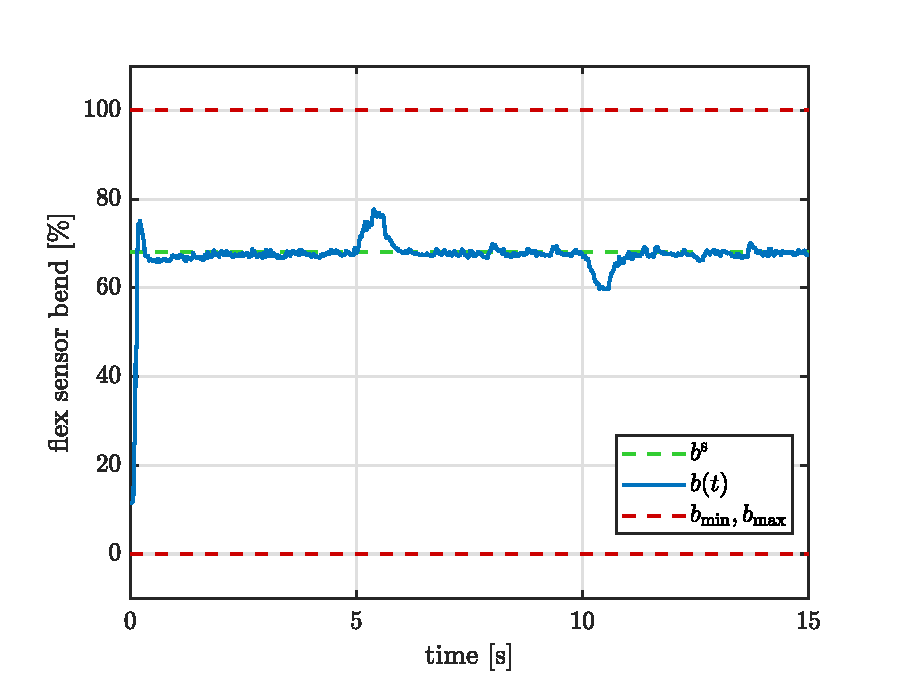
\includegraphics[width=0.5\textwidth]{images/deltaU_b_new.eps}
		\caption{Tube MPC with rate constraints. Trajectory of controlled variable.}
		\label{fig:deltaU_y}
	\end{center}
	%\end{figure}
	%
	%\begin{figure}
	\begin{center}
		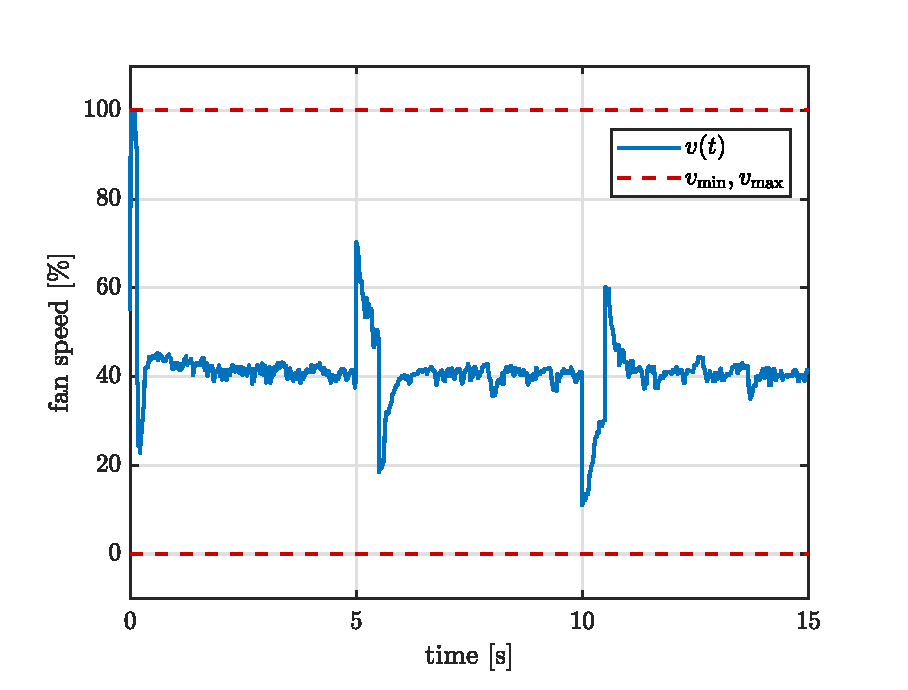
\includegraphics[width=0.5\textwidth]{images/deltaU_v_new.eps}
		\caption{Tube MPC with rate constraints. Trajectory of manipulated variable.}
		\label{fig:deltaU_u}
	\end{center}
\end{figure}

This section addresses the experimental implementation of the two presented control methods, i.e., the Tube explicit MPC with rate constraints, and polynomial approximation of an explicit MPC controller. To provide experimental results presenting the proposed methods, the case study was realized on a dynamical SISO device Flexy2~\cite{flexy2}, see Figure~\ref{fig:flexy2}. The actuator is a fan that propels an air column in an upward vertical direction. The power of the airflow is measured
by a flexible sensor placed in the air column. The sensor changes its electrical resistance according to the bend caused by the push of the air. Therefore, the flex sensor bend $b(t)$ in percentage is assumed as the controlled variable, and the fan speed $v(t)$ in percentage is a manipulated variable.

Flexy2 is a system with non-linear dynamics, as the sensitivity of the flex bend decreases when increasing fan speed. Moreover, the oscillations are minor at higher fan speed. Lastly, the measurement noise is also present. These challenges make this device a suitable candidate for the implementation of Tube MPC. As the system is naturally very fast and requires low sampling time with fast evaluation of the control inputs, the explicit solution of Tube MPC is considered. In this paper, the goal was to control the flex sensor bend $b(t)$ to a steady-state value $b^\text{s}$ and reject effect of a disturbance $d(t)$.

\begin{figure}
	\begin{center}
		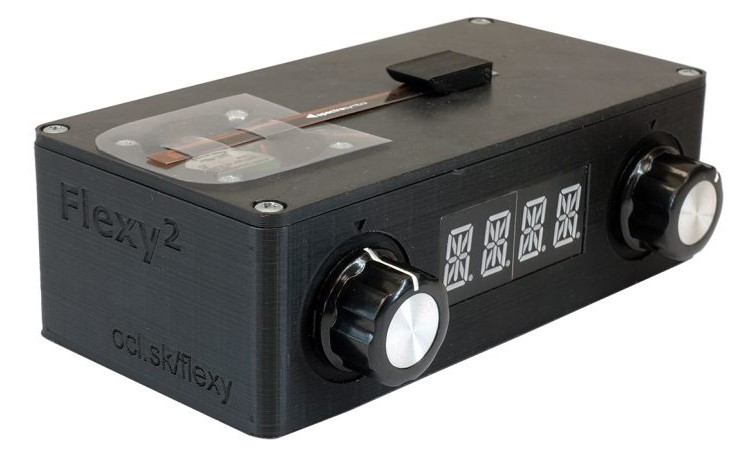
\includegraphics[width=0.35\textwidth]{images/flexy2}
		\caption{Flexy2 device~\cite{flexy2}.}
		\label{fig:flexy2}
	\end{center}
\end{figure}

The model of the system was obtained through experimental identification based on several step responses. The matrices of the nominal state-space system, transformed into the discrete-time domain using sampling time $T_\mathrm{s} = 0.01$\,s are:
\begin{equation}
	\label{eq:model_A_B} 
		A = \begin{bmatrix}
			0.966
		\end{bmatrix}, \quad 
		B = \begin{bmatrix}
			0.101
		\end{bmatrix}. 
\end{equation}

As the controlled as well as the manipulated variable were set in percentage, their values were constrained from $b_{\min} = v_{\min} = 0\%$ to $b_{\max} = v_{\max} = 100\,\%$. Considering the steady-state values where the model was linearized, i.e., $ v^\mathrm{s} = 40\%$ and $ b^\mathrm{s} = 68\%$, the constraints were set in both presented control methods as follows: 
\begin{eqnarray}
\label{eq:const_u_y}
	-40\,\% \le u(t) \le 60\,\%, \quad -68\,\% \le x(t) \le 32\,\%.
\end{eqnarray}

The rest of the two explicit MPC setups is described in the follow up sections, according to the specific control approach, as the controllers differ in their structures and tuning parameters. Both explicit MPC feedback laws~\eqref{eq:tmpc_control_law_pwa} were constructed in \texttt{MATLAB 2020b} programming environment, using toolboxes  \texttt{MPT 3.2.1}, \texttt{MPTplus}, \texttt{YALMIP R20210331},
and solver \texttt{Gurobi 9.1.1}. The explicit MPCs were executed on
CPU \texttt{AMD Ryzen 7 PRO 4750U}, 1.7\,GHz with 16\,GB RAM. 
We would like to note that, due to the paper limitations, all \texttt{MPTplus} commands are here omitted.\footnote{Interested readers are refereed to \url{https://github.com/holaza/mptplus/wiki} for a more detailed guidance on how to use \texttt{MPTplus} framework.}

%It should be emphasize that all explicit feedback laws~\eqref{eq:tmpc_control_law_pwa} in this Section were constructed and evaluated with the ease of \texttt{MPTplus} framework, i.e. by using user-friendly commands described in Section~\ref{sec:explicit_mpc}. However, due to the paper limitations, these commands are omitted.\footnote{Interested readers are refereed to \url{https://github.com/holaza/mptplus/wiki} for a more detailed guidance on how to use \texttt{MPTplus} framework.}


\subsection{Tube explicit MPC with rate constraints}
\label{sec:tube_exp}

In this section, the implementation of Tube explicit MPC with rate constraints is described. Let us consider the system model in~\eqref{eq:model_A_B} and constraints stated in~\eqref{eq:const_du}. 
As the uncertainties in the model were considered, the additive disturbance was considered in the MPC design as well and was constrained as:
\begin{eqnarray}
	\label{eq:const_w}
	-1\,\% \le w(t) \le 1\,\%.
\end{eqnarray}

Moreover, the change of the input variable was set to validate the control method implemented in the toolbox:
\begin{eqnarray}
	\label{eq:const_du}
	-55\,\% \le \Delta u \le 55\,\%.
\end{eqnarray}
By systematic tuning, the penalty matrices $Q$, $R$ of the optimization problem in~\eqref{eq:tmpc}, and the terminal penalty $P$ given by the LQR penalty, were respectively assigned as:
\begin{eqnarray}
\label{eq:setup_penalty}
Q = 10, \quad R = 1, \quad P = 95.3852 \, .
\end{eqnarray}

%The terminal penalty matrix $P$ was set as the LQR penalty, i.e.:
%\begin{eqnarray}
%	\label{eq:setup_P}
%	P = 95.3852.
%\end{eqnarray}
Furthermore, the terminal set was constructed as the LQR set and was defined by the following inequality:
\begin{eqnarray}
	\label{eq:setup_terminal_set}
	\begin{bmatrix}
	-1 \\	
	\,\,\,\,\, 1
	\end{bmatrix} x \le 
	\begin{bmatrix}
		31.8694\\	
		21.2463
	\end{bmatrix}.
\end{eqnarray}
The prediction horizon $N$ was set to 30 steps. 
%The associated explicit MPC policy was constructed via \texttt{MPTplus} framework by execution several lines of code as described in Section~\ref{sec:explicit_mpc}. The resulting feedback law~\eqref{eq:tmpc_control_law_pwa} consisted of $n_\text{r} = 12$ critical regions.
After the construction of the Tube explicit model predictive controller, the disturbance rejection control problem was investigated. The control results can be seen in Figure~\ref{fig:deltaU_y} for the controlled variable, i.e., the flex sensor bend $b(t)$. In Figure~\ref{fig:deltaU_u}, the corresponding trajectory of manipulated variable is depicted, i.e., the trajectory of fan speed $v(t)$. The aim was to drive the flex sensor bend to the steady state $ b^\mathrm{s} = 68\%$, while rejecting the effect of the two disturbances occurring at times 5\,s and 10\,s. 

When observing Figures~\ref{fig:deltaU_y}, \ref{fig:deltaU_u}, it can be seen that the goal of the control was achieved. The effects of both disturbances were rejected, with respect to the constraints on the manipulated and controlled variables. Moreover, the constraints on the change of the manipulated variable were satisfied as well.

\subsection{Polynomial approximation of explicit MPC}
\label{sec:polynomial_exp}

\begin{figure}[bp!]
	\begin{center}
		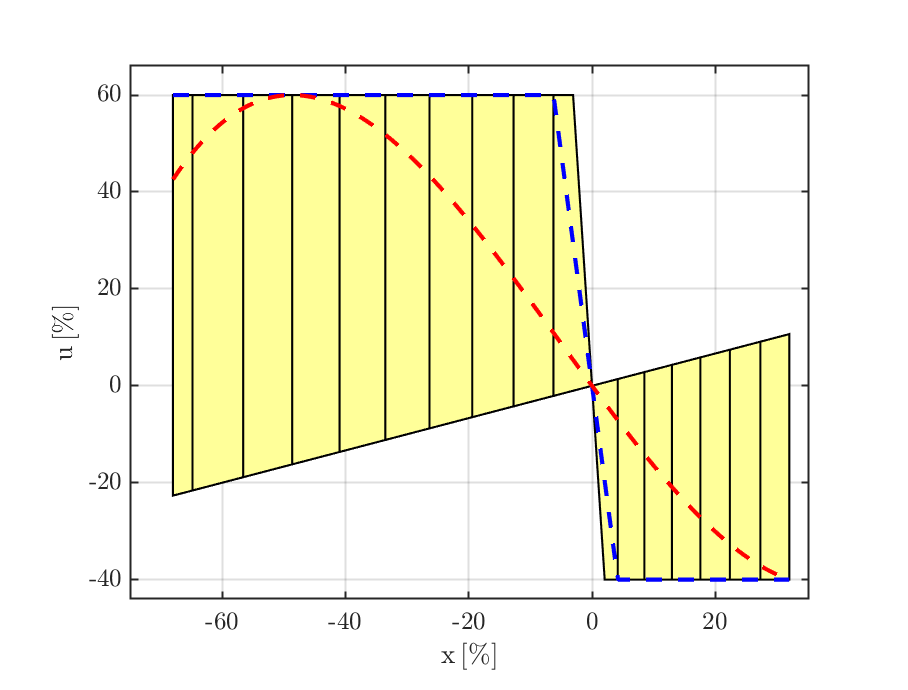
\includegraphics[width=0.5\textwidth]{images/approximation.eps}
		\caption{Approximation of the optimal explicit Tube MPC. The blue line represents the optimal control law, the yellow area is stability tube, and the red line represents the polynomial approximation of the optimal control law.}
		\label{fig:approx}
	\end{center}
\end{figure}

The following case study focuses on the second contribution of this paper, i.e., the implementation of the explicit control law approximated by a polynomial function as in~\eqref{eq:poly_control_law}. 
%
In this section we have assumed MPC setup as in~\eqref{eq:empc} with one-norm $p = 1$, prediction horizon $N = 10$, model~\eqref{eq:model_A_B}, state and input constraints~\eqref{eq:const_u_y}. The weighting matrices were set to $Q = 10$ and $R = 1$.
%
The resulting explicit feedback law~\eqref{eq:tmpc_control_law_pwa} was defined over polyhedral partition consisting of $17$ critical regions.

Next, the polynomial controller~\eqref{eq:poly_control_law} was created based on the optimal one. The degree of the polynomial was set to $\polydegree = 3$ and all other optional parameters were kept to their default values. The approximation of the optimal control law can be seen in Figure~\ref{fig:approx}.




%Let us consider the system model in~\eqref{eq:model_A_B} and constraints stated in~\eqref{eq:const_du}. By systematic tuning, the penalty matrices of the optimization problem in~\eqref{eq:empc_cost} were set as:	
%\begin{eqnarray}
%\label{eq:setup_penalty_pol} 
%	Q = 10, \quad R = 1.
%\end{eqnarray}

\begin{figure}[bp!]
	\begin{center}
		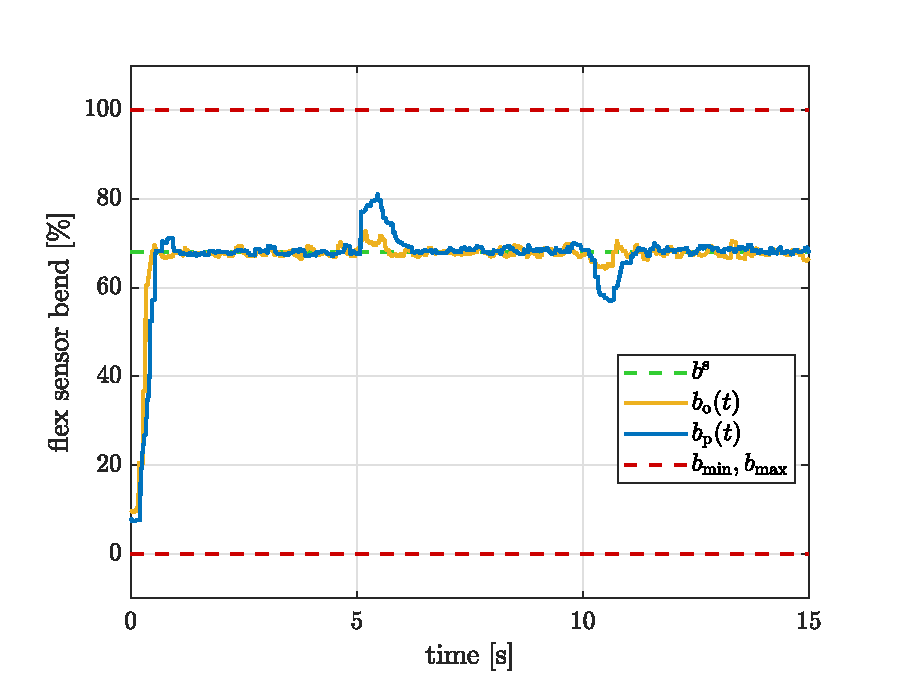
\includegraphics[width=0.5\textwidth]{images/poly_b.eps}
		\caption{Comparison of optimal explicit Tube MPC and its polynomial approximation: trajectory of controlled variable.}
		\label{fig:poly_y}
	\end{center}
	%\end{figure}
	%
	%\begin{figure}
	\begin{center}
		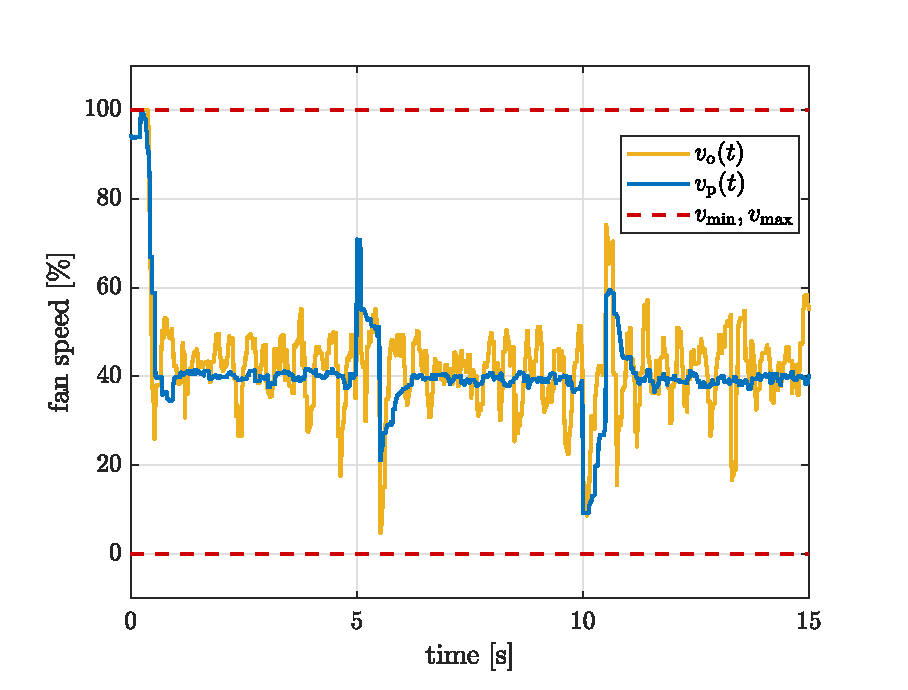
\includegraphics[width=0.5\textwidth]{images/poly_v.eps}
		\caption{Comparison of optimal explicit Tube MPC and its polynomial approximation: trajectory of manipulated variable.}
		\label{fig:poly_u}
	\end{center}
\end{figure}

%The prediction horizon was set as 10 steps long. Based on the aforementioned parameters, the explicit MPC was constructed. Next, the polynomial controller was created based on the optimal one. The degree of the polynomial was determined to 3\textsuperscript{rd} degree. The approximation of the optimal control law can be seen in Figure~\ref{fig:approx}.

The comparison of the control results can be seen in Figure~\ref{fig:poly_y} for the controlled variable and in Figure~\ref{fig:poly_u} for the manipulated input. In both graphs, two trajectories are depicted - for the original optimal controller with subscript ``o'' and its polynomial approximation with subscpript ``p''. Analogously to the first case study, the aim was to drive the flex sensor bend to the steady state $ b^\mathrm{s} = 68\,\%$, while rejecting the effect of the two disturbances occurring at times 5\,s and 10\,s.

It can be seen in Figure~\ref{fig:poly_y}, that both disturbances were successfully rejected. Compared to the optimal controller, the approximated one was less oscillating in terms of manipulated variable, see Figure~\ref{fig:poly_u}. With more cautious control inputs, the effect of the disturbance on the trajectory of controlled variable is more significant. The reason of less oscillating control inputs can be seen in Figure~\ref{fig:approx}. The original PWA control law is more steep around the origin, while the polynomial approximation is quite moderate. The approximation can be further tuned by setting the polynomial order, which, obviously, directly affects the control performance.


\section{Conclusions}
\label{sec:conclusions}

% [ TOOD: Summarize the main conclusions. ]
The paper presented a detailed tutorial for package \texttt{MPTplus} extending the original \texttt{MPT} toolbox. Among other relevant features, the release introduces the full framework for the memory-efficient explicit Tube MPC design taking into account also the limited rate of control action. \texttt{MPT} toolbox also enables the construction of light-weight polynomial-approximation-based controllers. The possibilities of construction, tuning, and validation of the various MPC controllers were analyzed by the laboratory implementation on the device with fast dynamics. The measured control profiles confirmed the ease of MPC tuning and the benefits of the user-friendly environment of \texttt{MPTplus} pushing the designed MPC controllers towards their industrial implementation.

\addtolength{\textheight}{-12cm}

\section*{Acknowledgemnts}

% [ TODO: Double-check Acks. ]
\small{
This research is funded by the European Commission under the grant no. 101079342 (Fostering Opportunities Towards Slovak Excellence in Advanced Control for Smart Industries). The authors gratefully acknowledge the contribution of the Scientific Grant Agency of the Slovak Republic under the grants 1/0545/20, 1/0297/22, and the Slovak Research and Development Agency under the project APVV-20-0261. L. Galčíková was also supported by an internal STU grant. 
}

\bibliographystyle{IEEEtran}
% \small
\bibliography{references}


\end{document}
